\section{Open-loop system}

In situations where a system is open-loop unstable, conducting experiments directly on the open-loop system can be challenging or even impossible due to the inherent instability. 
However, one approach to analyze and identify the system's characteristics is to perform a closed-loop experiment.

In a closed-loop experiment, the system is stabilized by feedback, allowing for safe and controlled data collection. 
The feedback loop ensures that the output of the system is regulated and can be measured accurately. 
This setup enables the collection of data for system identification and analysis.
\begin{figure}[H]
    \centering
    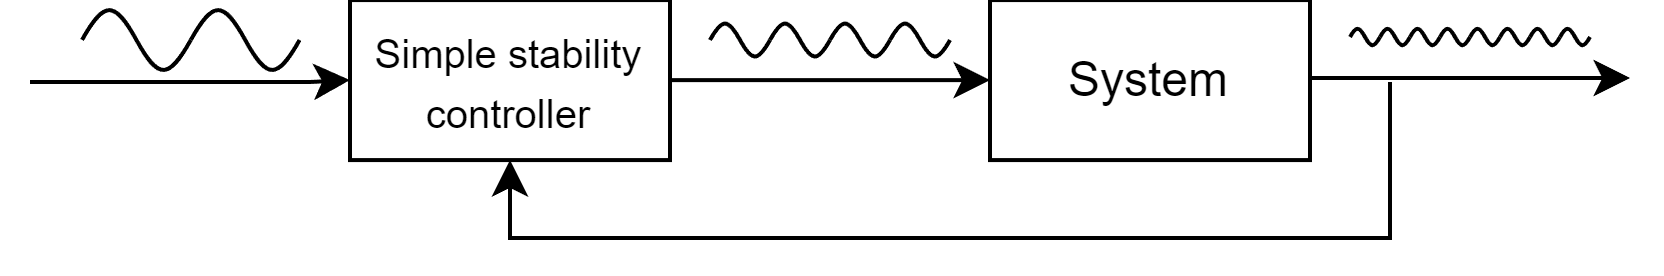
\includegraphics[width=0.6\linewidth]{images/cle.png}
    \caption{Closed-loop system identification}
\end{figure}
By performing experiments in a closed-loop configuration, it is possible to study and understand the behavior of unstable systems while maintaining stability and safety.
This approach is commonly used in control system analysis and design, particularly when dealing with unstable or uncertain systems.